\documentclass{standalone}
\usepackage{tikz}
\usetikzlibrary{patterns, positioning}

\begin{document}
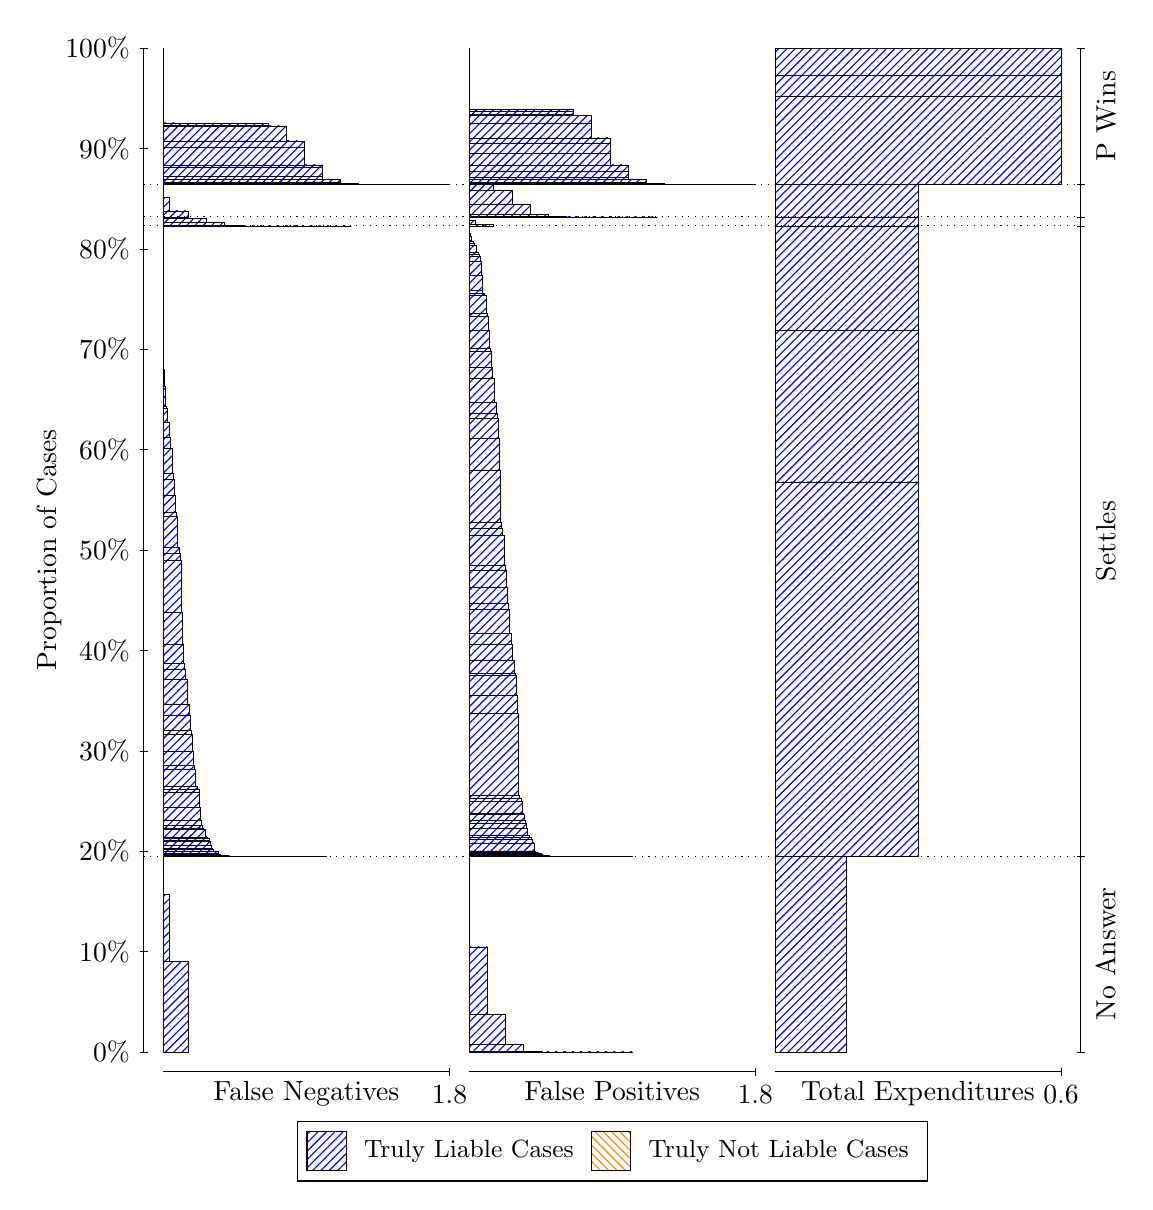
\begin{tikzpicture}
\draw[black, very thin] (1.5,1.75) -- (1.5,14.5);
\node[rotate=90, anchor=center] at (0.3, 8.125) {Proportion of Cases};
\draw[black, very thin] (1.45,1.75) -- (1.55,1.75);
\node[anchor=east] at (1.45, 1.75) {0\%};
\draw[black, very thin] (1.45,3.025) -- (1.55,3.025);
\node[anchor=east] at (1.45, 3.025) {10\%};
\draw[black, very thin] (1.45,4.3) -- (1.55,4.3);
\node[anchor=east] at (1.45, 4.3) {20\%};
\draw[black, very thin] (1.45,5.575) -- (1.55,5.575);
\node[anchor=east] at (1.45, 5.575) {30\%};
\draw[black, very thin] (1.45,6.85) -- (1.55,6.85);
\node[anchor=east] at (1.45, 6.85) {40\%};
\draw[black, very thin] (1.45,8.125) -- (1.55,8.125);
\node[anchor=east] at (1.45, 8.125) {50\%};
\draw[black, very thin] (1.45,9.4) -- (1.55,9.4);
\node[anchor=east] at (1.45, 9.4) {60\%};
\draw[black, very thin] (1.45,10.675) -- (1.55,10.675);
\node[anchor=east] at (1.45, 10.675) {70\%};
\draw[black, very thin] (1.45,11.95) -- (1.55,11.95);
\node[anchor=east] at (1.45, 11.95) {80\%};
\draw[black, very thin] (1.45,13.225) -- (1.55,13.225);
\node[anchor=east] at (1.45, 13.225) {90\%};
\draw[black, very thin] (1.45,14.5) -- (1.55,14.5);
\node[anchor=east] at (1.45, 14.5) {100\%};

\draw[black, very thin] (13.4,1.75) -- (13.4,14.5);
\draw[black, very thin] (13.35,1.75) -- (13.45,1.75);
\node[anchor=west] at (13.35, 1.75) {};
\draw[black, very thin] (13.35,4.2363) -- (13.45,4.2363);
\node[anchor=west] at (13.35, 4.2363) {};
\draw[black, very thin] (13.35,12.242) -- (13.45,12.242);
\node[anchor=west] at (13.35, 12.242) {};
\draw[black, very thin] (13.35,12.356) -- (13.45,12.356);
\node[anchor=west] at (13.35, 12.356) {};
\draw[black, very thin] (13.35,12.766) -- (13.45,12.766);
\node[anchor=west] at (13.35, 12.766) {};
\draw[black, very thin] (13.35,14.5) -- (13.45,14.5);
\node[anchor=west] at (13.35, 14.5) {};

\draw[black, very thin, pattern color=blue, pattern=north east lines] (1.75,1.75) rectangle (2.0614,2.9018);
\draw[black, very thin, pattern color=blue, pattern=north east lines] (1.75,2.9018) rectangle (1.8307,3.7553);
\draw[black, very thin, pattern color=orange, pattern=north west lines] (1.75,3.7553) rectangle (1.75,3.7553);
\draw[black, very thin, pattern color=blue, pattern=north east lines] (1.75,3.7553) rectangle (1.75,4.2363);
\draw[black, very thin, pattern color=blue, pattern=north east lines] (1.75,4.2363) rectangle (3.8262,4.2363);
\draw[black, very thin, pattern color=blue, pattern=north east lines] (1.75,4.2363) rectangle (3.7224,4.2363);
\draw[black, very thin, pattern color=blue, pattern=north east lines] (1.75,4.2363) rectangle (3.6186,4.2363);
\draw[black, very thin, pattern color=blue, pattern=north east lines] (1.75,4.2363) rectangle (3.5955,4.2363);
\draw[black, very thin, pattern color=blue, pattern=north east lines] (1.75,4.2363) rectangle (3.5148,4.2363);
\draw[black, very thin, pattern color=blue, pattern=north east lines] (1.75,4.2363) rectangle (3.4917,4.2363);
\draw[black, very thin, pattern color=blue, pattern=north east lines] (1.75,4.2363) rectangle (3.411,4.2363);
\draw[black, very thin, pattern color=blue, pattern=north east lines] (1.75,4.2363) rectangle (3.3879,4.2363);
\draw[black, very thin, pattern color=blue, pattern=north east lines] (1.75,4.2363) rectangle (3.3648,4.2363);
\draw[black, very thin, pattern color=blue, pattern=north east lines] (1.75,4.2363) rectangle (3.3071,4.2363);
\draw[black, very thin, pattern color=blue, pattern=north east lines] (1.75,4.2363) rectangle (3.2841,4.2363);
\draw[black, very thin, pattern color=blue, pattern=north east lines] (1.75,4.2363) rectangle (3.261,4.2363);
\draw[black, very thin, pattern color=blue, pattern=north east lines] (1.75,4.2363) rectangle (3.2033,4.2363);
\draw[black, very thin, pattern color=blue, pattern=north east lines] (1.75,4.2363) rectangle (3.1803,4.2363);
\draw[black, very thin, pattern color=blue, pattern=north east lines] (1.75,4.2363) rectangle (3.1572,4.2363);
\draw[black, very thin, pattern color=blue, pattern=north east lines] (1.75,4.2363) rectangle (3.1341,4.2363);
\draw[black, very thin, pattern color=blue, pattern=north east lines] (1.75,4.2363) rectangle (3.0995,4.2363);
\draw[black, very thin, pattern color=blue, pattern=north east lines] (1.75,4.2363) rectangle (3.0765,4.2363);
\draw[black, very thin, pattern color=blue, pattern=north east lines] (1.75,4.2363) rectangle (3.0534,4.2363);
\draw[black, very thin, pattern color=blue, pattern=north east lines] (1.75,4.2363) rectangle (3.0303,4.2363);
\draw[black, very thin, pattern color=blue, pattern=north east lines] (1.75,4.2363) rectangle (2.9957,4.2363);
\draw[black, very thin, pattern color=blue, pattern=north east lines] (1.75,4.2363) rectangle (2.9726,4.2363);
\draw[black, very thin, pattern color=blue, pattern=north east lines] (1.75,4.2363) rectangle (2.9496,4.2363);
\draw[black, very thin, pattern color=blue, pattern=north east lines] (1.75,4.2363) rectangle (2.9265,4.2363);
\draw[black, very thin, pattern color=blue, pattern=north east lines] (1.75,4.2363) rectangle (2.9034,4.2363);
\draw[black, very thin, pattern color=blue, pattern=north east lines] (1.75,4.2363) rectangle (2.8919,4.2363);
\draw[black, very thin, pattern color=blue, pattern=north east lines] (1.75,4.2363) rectangle (2.8688,4.2363);
\draw[black, very thin, pattern color=blue, pattern=north east lines] (1.75,4.2363) rectangle (2.8458,4.2363);
\draw[black, very thin, pattern color=blue, pattern=north east lines] (1.75,4.2363) rectangle (2.8227,4.2363);
\draw[black, very thin, pattern color=blue, pattern=north east lines] (1.75,4.2363) rectangle (2.7996,4.2363);
\draw[black, very thin, pattern color=blue, pattern=north east lines] (1.75,4.2363) rectangle (2.7881,4.2363);
\draw[black, very thin, pattern color=blue, pattern=north east lines] (1.75,4.2363) rectangle (2.765,4.2363);
\draw[black, very thin, pattern color=blue, pattern=north east lines] (1.75,4.2363) rectangle (2.742,4.2364);
\draw[black, very thin, pattern color=blue, pattern=north east lines] (1.75,4.2364) rectangle (2.7189,4.2364);
\draw[black, very thin, pattern color=blue, pattern=north east lines] (1.75,4.2364) rectangle (2.6958,4.2364);
\draw[black, very thin, pattern color=blue, pattern=north east lines] (1.75,4.2364) rectangle (2.6843,4.237);
\draw[black, very thin, pattern color=blue, pattern=north east lines] (1.75,4.237) rectangle (2.6728,4.2373);
\draw[black, very thin, pattern color=blue, pattern=north east lines] (1.75,4.2373) rectangle (2.6612,4.2374);
\draw[black, very thin, pattern color=blue, pattern=north east lines] (1.75,4.2374) rectangle (2.6381,4.2374);
\draw[black, very thin, pattern color=blue, pattern=north east lines] (1.75,4.2374) rectangle (2.6151,4.238);
\draw[black, very thin, pattern color=blue, pattern=north east lines] (1.75,4.238) rectangle (2.592,4.2396);
\draw[black, very thin, pattern color=blue, pattern=north east lines] (1.75,4.2396) rectangle (2.5805,4.2442);
\draw[black, very thin, pattern color=blue, pattern=north east lines] (1.75,4.2442) rectangle (2.5689,4.2445);
\draw[black, very thin, pattern color=blue, pattern=north east lines] (1.75,4.2445) rectangle (2.5574,4.2451);
\draw[black, very thin, pattern color=blue, pattern=north east lines] (1.75,4.2451) rectangle (2.5343,4.2457);
\draw[black, very thin, pattern color=blue, pattern=north east lines] (1.75,4.2457) rectangle (2.5113,4.2509);
\draw[black, very thin, pattern color=blue, pattern=north east lines] (1.75,4.2509) rectangle (2.4882,4.2514);
\draw[black, very thin, pattern color=blue, pattern=north east lines] (1.75,4.2514) rectangle (2.4767,4.2548);
\draw[black, very thin, pattern color=blue, pattern=north east lines] (1.75,4.2548) rectangle (2.4651,4.2581);
\draw[black, very thin, pattern color=blue, pattern=north east lines] (1.75,4.2581) rectangle (2.4536,4.2758);
\draw[black, very thin, pattern color=blue, pattern=north east lines] (1.75,4.2758) rectangle (2.4421,4.2927);
\draw[black, very thin, pattern color=blue, pattern=north east lines] (1.75,4.2927) rectangle (2.4305,4.2961);
\draw[black, very thin, pattern color=blue, pattern=north east lines] (1.75,4.2961) rectangle (2.4075,4.298);
\draw[black, very thin, pattern color=blue, pattern=north east lines] (1.75,4.298) rectangle (2.3844,4.3242);
\draw[black, very thin, pattern color=blue, pattern=north east lines] (1.75,4.3242) rectangle (2.3729,4.3337);
\draw[black, very thin, pattern color=blue, pattern=north east lines] (1.75,4.3337) rectangle (2.3613,4.3701);
\draw[black, very thin, pattern color=blue, pattern=north east lines] (1.75,4.3701) rectangle (2.3498,4.4268);
\draw[black, very thin, pattern color=blue, pattern=north east lines] (1.75,4.4268) rectangle (2.3383,4.4338);
\draw[black, very thin, pattern color=blue, pattern=north east lines] (1.75,4.4338) rectangle (2.3267,4.4589);
\draw[black, very thin, pattern color=blue, pattern=north east lines] (1.75,4.4589) rectangle (2.3037,4.4815);
\draw[black, very thin, pattern color=blue, pattern=north east lines] (1.75,4.4815) rectangle (2.2806,4.5761);
\draw[black, very thin, pattern color=blue, pattern=north east lines] (1.75,4.5761) rectangle (2.2575,4.595);
\draw[black, very thin, pattern color=blue, pattern=north east lines] (1.75,4.595) rectangle (2.246,4.6246);
\draw[black, very thin, pattern color=blue, pattern=north east lines] (1.75,4.6246) rectangle (2.2344,4.6889);
\draw[black, very thin, pattern color=blue, pattern=north east lines] (1.75,4.6889) rectangle (2.2229,4.8585);
\draw[black, very thin, pattern color=blue, pattern=north east lines] (1.75,4.8585) rectangle (2.2114,5.0522);
\draw[black, very thin, pattern color=blue, pattern=north east lines] (1.75,5.0522) rectangle (2.1998,5.0922);
\draw[black, very thin, pattern color=blue, pattern=north east lines] (1.75,5.0922) rectangle (2.1768,5.1229);
\draw[black, very thin, pattern color=blue, pattern=north east lines] (1.75,5.1229) rectangle (2.1537,5.3464);
\draw[black, very thin, pattern color=blue, pattern=north east lines] (1.75,5.3464) rectangle (2.1422,5.3874);
\draw[black, very thin, pattern color=blue, pattern=north east lines] (1.75,5.3874) rectangle (2.1306,5.5658);
\draw[black, very thin, pattern color=blue, pattern=north east lines] (1.75,5.5658) rectangle (2.1191,5.7898);
\draw[black, very thin, pattern color=blue, pattern=north east lines] (1.75,5.7898) rectangle (2.1076,5.8303);
\draw[black, very thin, pattern color=blue, pattern=north east lines] (1.75,5.8303) rectangle (2.096,6.0322);
\draw[black, very thin, pattern color=blue, pattern=north east lines] (1.75,6.0322) rectangle (2.073,6.172);
\draw[black, very thin, pattern color=blue, pattern=north east lines] (1.75,6.172) rectangle (2.0499,6.4807);
\draw[black, very thin, pattern color=blue, pattern=north east lines] (1.75,6.4807) rectangle (2.0268,6.6148);
\draw[black, very thin, pattern color=blue, pattern=north east lines] (1.75,6.6148) rectangle (2.0153,6.6802);
\draw[black, very thin, pattern color=blue, pattern=north east lines] (1.75,6.6802) rectangle (2.0038,6.934);
\draw[black, very thin, pattern color=blue, pattern=north east lines] (1.75,6.934) rectangle (1.9922,7.3362);
\draw[black, very thin, pattern color=blue, pattern=north east lines] (1.75,7.3362) rectangle (1.9807,7.9964);
\draw[black, very thin, pattern color=blue, pattern=north east lines] (1.75,7.9964) rectangle (1.9692,8.0827);
\draw[black, very thin, pattern color=blue, pattern=north east lines] (1.75,8.0827) rectangle (1.9461,8.1639);
\draw[black, very thin, pattern color=blue, pattern=north east lines] (1.75,8.1639) rectangle (1.923,8.5536);
\draw[black, very thin, pattern color=blue, pattern=north east lines] (1.75,8.5536) rectangle (1.9115,8.6068);
\draw[black, very thin, pattern color=blue, pattern=north east lines] (1.75,8.6068) rectangle (1.8999,8.8221);
\draw[black, very thin, pattern color=blue, pattern=north east lines] (1.75,8.8221) rectangle (1.8884,9.0262);
\draw[black, very thin, pattern color=blue, pattern=north east lines] (1.75,9.0262) rectangle (1.8769,9.1004);
\draw[black, very thin, pattern color=blue, pattern=north east lines] (1.75,9.1004) rectangle (1.8653,9.4146);
\draw[black, very thin, pattern color=blue, pattern=north east lines] (1.75,9.4146) rectangle (1.8423,9.554);
\draw[black, very thin, pattern color=blue, pattern=north east lines] (1.75,9.554) rectangle (1.8192,9.7483);
\draw[black, very thin, pattern color=blue, pattern=north east lines] (1.75,9.7483) rectangle (1.7961,9.921);
\draw[black, very thin, pattern color=blue, pattern=north east lines] (1.75,9.921) rectangle (1.7846,9.9468);
\draw[black, very thin, pattern color=blue, pattern=north east lines] (1.75,9.9468) rectangle (1.7731,10.204);
\draw[black, very thin, pattern color=blue, pattern=north east lines] (1.75,10.204) rectangle (1.7615,10.421);
\draw[black, very thin, pattern color=orange, pattern=north west lines] (1.75,10.421) rectangle (1.75,10.421);
\draw[black, very thin, pattern color=blue, pattern=north east lines] (1.75,10.421) rectangle (1.75,12.242);
\draw[black, very thin, pattern color=blue, pattern=north east lines] (1.75,12.242) rectangle (4.1376,12.242);
\draw[black, very thin, pattern color=blue, pattern=north east lines] (1.75,12.242) rectangle (3.9069,12.242);
\draw[black, very thin, pattern color=blue, pattern=north east lines] (1.75,12.242) rectangle (3.6762,12.242);
\draw[black, very thin, pattern color=blue, pattern=north east lines] (1.75,12.242) rectangle (3.4456,12.242);
\draw[black, very thin, pattern color=blue, pattern=north east lines] (1.75,12.242) rectangle (3.2149,12.242);
\draw[black, very thin, pattern color=blue, pattern=north east lines] (1.75,12.242) rectangle (2.9842,12.242);
\draw[black, very thin, pattern color=blue, pattern=north east lines] (1.75,12.242) rectangle (2.7535,12.248);
\draw[black, very thin, pattern color=blue, pattern=north east lines] (1.75,12.248) rectangle (2.5228,12.284);
\draw[black, very thin, pattern color=blue, pattern=north east lines] (1.75,12.284) rectangle (2.2921,12.334);
\draw[black, very thin, pattern color=blue, pattern=north east lines] (1.75,12.334) rectangle (2.0614,12.356);
\draw[black, very thin, pattern color=orange, pattern=north west lines] (1.75,12.356) rectangle (1.75,12.356);
\draw[black, very thin, pattern color=blue, pattern=north east lines] (1.75,12.356) rectangle (2.0614,12.433);
\draw[black, very thin, pattern color=blue, pattern=north east lines] (1.75,12.433) rectangle (1.8307,12.606);
\draw[black, very thin, pattern color=orange, pattern=north west lines] (1.75,12.606) rectangle (1.75,12.606);
\draw[black, very thin, pattern color=blue, pattern=north east lines] (1.75,12.606) rectangle (1.75,12.766);
\draw[black, very thin, pattern color=blue, pattern=north east lines] (1.75,12.766) rectangle (5.3833,12.766);
\draw[black, very thin, pattern color=blue, pattern=north east lines] (1.75,12.766) rectangle (5.1526,12.766);
\draw[black, very thin, pattern color=blue, pattern=north east lines] (1.75,12.766) rectangle (4.922,12.766);
\draw[black, very thin, pattern color=blue, pattern=north east lines] (1.75,12.766) rectangle (4.6913,12.766);
\draw[black, very thin, pattern color=blue, pattern=north east lines] (1.75,12.766) rectangle (4.6913,12.766);
\draw[black, very thin, pattern color=blue, pattern=north east lines] (1.75,12.766) rectangle (4.4606,12.767);
\draw[black, very thin, pattern color=blue, pattern=north east lines] (1.75,12.767) rectangle (4.4606,12.767);
\draw[black, very thin, pattern color=blue, pattern=north east lines] (1.75,12.767) rectangle (4.2299,12.778);
\draw[black, very thin, pattern color=blue, pattern=north east lines] (1.75,12.778) rectangle (3.9992,12.8);
\draw[black, very thin, pattern color=blue, pattern=north east lines] (1.75,12.8) rectangle (3.9992,12.834);
\draw[black, very thin, pattern color=blue, pattern=north east lines] (1.75,12.834) rectangle (3.7685,12.869);
\draw[black, very thin, pattern color=blue, pattern=north east lines] (1.75,12.869) rectangle (3.7685,12.991);
\draw[black, very thin, pattern color=blue, pattern=north east lines] (1.75,12.991) rectangle (3.7685,13.016);
\draw[black, very thin, pattern color=blue, pattern=north east lines] (1.75,13.016) rectangle (3.5378,13.235);
\draw[black, very thin, pattern color=blue, pattern=north east lines] (1.75,13.235) rectangle (3.5378,13.32);
\draw[black, very thin, pattern color=blue, pattern=north east lines] (1.75,13.32) rectangle (3.3071,13.512);
\draw[black, very thin, pattern color=blue, pattern=north east lines] (1.75,13.512) rectangle (3.0765,13.513);
\draw[black, very thin, pattern color=blue, pattern=north east lines] (1.75,13.513) rectangle (3.0765,13.544);
\draw[black, very thin, pattern color=blue, pattern=north east lines] (1.75,13.544) rectangle (3.0534,13.544);
\draw[black, very thin, pattern color=blue, pattern=north east lines] (1.75,13.544) rectangle (2.8458,13.545);
\draw[black, very thin, pattern color=blue, pattern=north east lines] (1.75,13.545) rectangle (2.8458,13.545);
\draw[black, very thin, pattern color=blue, pattern=north east lines] (1.75,13.545) rectangle (2.8227,13.545);
\draw[black, very thin, pattern color=blue, pattern=north east lines] (1.75,13.545) rectangle (2.8227,13.545);
\draw[black, very thin, pattern color=blue, pattern=north east lines] (1.75,13.545) rectangle (2.6151,13.545);
\draw[black, very thin, pattern color=blue, pattern=north east lines] (1.75,13.545) rectangle (2.6151,13.545);
\draw[black, very thin, pattern color=blue, pattern=north east lines] (1.75,13.545) rectangle (2.592,13.545);
\draw[black, very thin, pattern color=blue, pattern=north east lines] (1.75,13.545) rectangle (2.592,13.545);
\draw[black, very thin, pattern color=blue, pattern=north east lines] (1.75,13.545) rectangle (2.592,13.545);
\draw[black, very thin, pattern color=blue, pattern=north east lines] (1.75,13.545) rectangle (2.3844,13.545);
\draw[black, very thin, pattern color=blue, pattern=north east lines] (1.75,13.545) rectangle (2.3844,13.545);
\draw[black, very thin, pattern color=blue, pattern=north east lines] (1.75,13.545) rectangle (2.3613,13.545);
\draw[black, very thin, pattern color=blue, pattern=north east lines] (1.75,13.545) rectangle (2.3613,13.545);
\draw[black, very thin, pattern color=blue, pattern=north east lines] (1.75,13.545) rectangle (2.1537,13.545);
\draw[black, very thin, pattern color=blue, pattern=north east lines] (1.75,13.545) rectangle (2.1537,13.545);
\draw[black, very thin, pattern color=blue, pattern=north east lines] (1.75,13.545) rectangle (2.1306,13.545);
\draw[black, very thin, pattern color=blue, pattern=north east lines] (1.75,13.545) rectangle (2.1306,13.545);
\draw[black, very thin, pattern color=blue, pattern=north east lines] (1.75,13.545) rectangle (2.1306,13.545);
\draw[black, very thin, pattern color=blue, pattern=north east lines] (1.75,13.545) rectangle (1.923,13.545);
\draw[black, very thin, pattern color=blue, pattern=north east lines] (1.75,13.545) rectangle (1.923,13.545);
\draw[black, very thin, pattern color=blue, pattern=north east lines] (1.75,13.545) rectangle (1.8999,13.546);
\draw[black, very thin, pattern color=blue, pattern=north east lines] (1.75,13.546) rectangle (1.8999,13.546);
\draw[black, very thin, pattern color=blue, pattern=north east lines] (1.75,13.546) rectangle (1.8999,13.549);
\draw[black, very thin, pattern color=orange, pattern=north west lines] (1.75,13.549) rectangle (1.75,13.549);
\draw[black, very thin, pattern color=blue, pattern=north east lines] (1.75,13.549) rectangle (1.75,14.5);
\draw[black, very thin, pattern color=orange, pattern=north west lines] (5.6333,1.75) rectangle (7.7095,1.75);
\draw[black, very thin, pattern color=blue, pattern=north east lines] (5.6333,1.75) rectangle (7.7095,1.75);
\draw[black, very thin, pattern color=blue, pattern=north east lines] (5.6333,1.75) rectangle (7.4788,1.75);
\draw[black, very thin, pattern color=blue, pattern=north east lines] (5.6333,1.75) rectangle (7.2481,1.75);
\draw[black, very thin, pattern color=blue, pattern=north east lines] (5.6333,1.75) rectangle (7.0175,1.75);
\draw[black, very thin, pattern color=blue, pattern=north east lines] (5.6333,1.75) rectangle (6.7868,1.7503);
\draw[black, very thin, pattern color=blue, pattern=north east lines] (5.6333,1.7503) rectangle (6.5561,1.7582);
\draw[black, very thin, pattern color=blue, pattern=north east lines] (5.6333,1.7582) rectangle (6.3254,1.8431);
\draw[black, very thin, pattern color=blue, pattern=north east lines] (5.6333,1.8431) rectangle (6.0947,2.231);
\draw[black, very thin, pattern color=blue, pattern=north east lines] (5.6333,2.231) rectangle (5.864,3.0845);
\draw[black, very thin, pattern color=blue, pattern=north east lines] (5.6333,3.0845) rectangle (5.6333,4.2363);
\draw[black, very thin, pattern color=orange, pattern=north west lines] (5.6333,4.2363) rectangle (7.7095,4.2363);
\draw[black, very thin, pattern color=blue, pattern=north east lines] (5.6333,4.2363) rectangle (7.7095,4.2363);
\draw[black, very thin, pattern color=orange, pattern=north west lines] (5.6333,4.2363) rectangle (7.6057,4.2363);
\draw[black, very thin, pattern color=blue, pattern=north east lines] (5.6333,4.2363) rectangle (7.6057,4.2363);
\draw[black, very thin, pattern color=orange, pattern=north west lines] (5.6333,4.2363) rectangle (7.5019,4.2363);
\draw[black, very thin, pattern color=blue, pattern=north east lines] (5.6333,4.2363) rectangle (7.5019,4.2363);
\draw[black, very thin, pattern color=blue, pattern=north east lines] (5.6333,4.2363) rectangle (7.4788,4.2363);
\draw[black, very thin, pattern color=orange, pattern=north west lines] (5.6333,4.2363) rectangle (7.3981,4.2363);
\draw[black, very thin, pattern color=blue, pattern=north east lines] (5.6333,4.2363) rectangle (7.3981,4.2363);
\draw[black, very thin, pattern color=blue, pattern=north east lines] (5.6333,4.2363) rectangle (7.375,4.2363);
\draw[black, very thin, pattern color=orange, pattern=north west lines] (5.6333,4.2363) rectangle (7.2943,4.2363);
\draw[black, very thin, pattern color=blue, pattern=north east lines] (5.6333,4.2363) rectangle (7.2943,4.2363);
\draw[black, very thin, pattern color=blue, pattern=north east lines] (5.6333,4.2363) rectangle (7.2712,4.2363);
\draw[black, very thin, pattern color=blue, pattern=north east lines] (5.6333,4.2363) rectangle (7.2481,4.2363);
\draw[black, very thin, pattern color=orange, pattern=north west lines] (5.6333,4.2363) rectangle (7.1905,4.2363);
\draw[black, very thin, pattern color=blue, pattern=north east lines] (5.6333,4.2363) rectangle (7.1905,4.2363);
\draw[black, very thin, pattern color=blue, pattern=north east lines] (5.6333,4.2363) rectangle (7.1674,4.2363);
\draw[black, very thin, pattern color=blue, pattern=north east lines] (5.6333,4.2363) rectangle (7.1443,4.2363);
\draw[black, very thin, pattern color=orange, pattern=north west lines] (5.6333,4.2363) rectangle (7.0867,4.2363);
\draw[black, very thin, pattern color=blue, pattern=north east lines] (5.6333,4.2363) rectangle (7.0867,4.2363);
\draw[black, very thin, pattern color=blue, pattern=north east lines] (5.6333,4.2363) rectangle (7.0636,4.2363);
\draw[black, very thin, pattern color=blue, pattern=north east lines] (5.6333,4.2363) rectangle (7.0405,4.2363);
\draw[black, very thin, pattern color=blue, pattern=north east lines] (5.6333,4.2363) rectangle (7.0175,4.2363);
\draw[black, very thin, pattern color=orange, pattern=north west lines] (5.6333,4.2363) rectangle (6.9829,4.2363);
\draw[black, very thin, pattern color=blue, pattern=north east lines] (5.6333,4.2363) rectangle (6.9829,4.2363);
\draw[black, very thin, pattern color=blue, pattern=north east lines] (5.6333,4.2363) rectangle (6.9598,4.2363);
\draw[black, very thin, pattern color=blue, pattern=north east lines] (5.6333,4.2363) rectangle (6.9367,4.2363);
\draw[black, very thin, pattern color=blue, pattern=north east lines] (5.6333,4.2363) rectangle (6.9137,4.2363);
\draw[black, very thin, pattern color=orange, pattern=north west lines] (5.6333,4.2363) rectangle (6.879,4.2363);
\draw[black, very thin, pattern color=blue, pattern=north east lines] (5.6333,4.2363) rectangle (6.879,4.2363);
\draw[black, very thin, pattern color=blue, pattern=north east lines] (5.6333,4.2363) rectangle (6.856,4.2363);
\draw[black, very thin, pattern color=blue, pattern=north east lines] (5.6333,4.2363) rectangle (6.8329,4.2364);
\draw[black, very thin, pattern color=blue, pattern=north east lines] (5.6333,4.2364) rectangle (6.8098,4.2364);
\draw[black, very thin, pattern color=blue, pattern=north east lines] (5.6333,4.2364) rectangle (6.7868,4.2364);
\draw[black, very thin, pattern color=orange, pattern=north west lines] (5.6333,4.2364) rectangle (6.7752,4.2364);
\draw[black, very thin, pattern color=blue, pattern=north east lines] (5.6333,4.2364) rectangle (6.7752,4.2368);
\draw[black, very thin, pattern color=blue, pattern=north east lines] (5.6333,4.2368) rectangle (6.7522,4.2369);
\draw[black, very thin, pattern color=blue, pattern=north east lines] (5.6333,4.2369) rectangle (6.7291,4.2369);
\draw[black, very thin, pattern color=blue, pattern=north east lines] (5.6333,4.2369) rectangle (6.706,4.2374);
\draw[black, very thin, pattern color=blue, pattern=north east lines] (5.6333,4.2374) rectangle (6.683,4.2374);
\draw[black, very thin, pattern color=orange, pattern=north west lines] (5.6333,4.2374) rectangle (6.6714,4.2374);
\draw[black, very thin, pattern color=blue, pattern=north east lines] (5.6333,4.2374) rectangle (6.6714,4.2415);
\draw[black, very thin, pattern color=blue, pattern=north east lines] (5.6333,4.2415) rectangle (6.6484,4.2421);
\draw[black, very thin, pattern color=blue, pattern=north east lines] (5.6333,4.2421) rectangle (6.6253,4.2427);
\draw[black, very thin, pattern color=blue, pattern=north east lines] (5.6333,4.2427) rectangle (6.6022,4.2479);
\draw[black, very thin, pattern color=blue, pattern=north east lines] (5.6333,4.2479) rectangle (6.5792,4.2494);
\draw[black, very thin, pattern color=orange, pattern=north west lines] (5.6333,4.2494) rectangle (6.5676,4.2494);
\draw[black, very thin, pattern color=blue, pattern=north east lines] (5.6333,4.2494) rectangle (6.5676,4.2603);
\draw[black, very thin, pattern color=blue, pattern=north east lines] (5.6333,4.2603) rectangle (6.5561,4.2611);
\draw[black, very thin, pattern color=blue, pattern=north east lines] (5.6333,4.2611) rectangle (6.5446,4.2755);
\draw[black, very thin, pattern color=blue, pattern=north east lines] (5.6333,4.2755) rectangle (6.5215,4.2784);
\draw[black, very thin, pattern color=blue, pattern=north east lines] (5.6333,4.2784) rectangle (6.4984,4.2804);
\draw[black, very thin, pattern color=blue, pattern=north east lines] (5.6333,4.2804) rectangle (6.4753,4.3049);
\draw[black, very thin, pattern color=orange, pattern=north west lines] (5.6333,4.3049) rectangle (6.4638,4.3049);
\draw[black, very thin, pattern color=blue, pattern=north east lines] (5.6333,4.3049) rectangle (6.4638,4.4048);
\draw[black, very thin, pattern color=blue, pattern=north east lines] (5.6333,4.4048) rectangle (6.4523,4.4064);
\draw[black, very thin, pattern color=blue, pattern=north east lines] (5.6333,4.4064) rectangle (6.4407,4.4541);
\draw[black, very thin, pattern color=blue, pattern=north east lines] (5.6333,4.4541) rectangle (6.4177,4.4779);
\draw[black, very thin, pattern color=blue, pattern=north east lines] (5.6333,4.4779) rectangle (6.3946,4.5003);
\draw[black, very thin, pattern color=blue, pattern=north east lines] (5.6333,4.5003) rectangle (6.3715,4.5949);
\draw[black, very thin, pattern color=orange, pattern=north west lines] (5.6333,4.5949) rectangle (6.36,4.5949);
\draw[black, very thin, pattern color=blue, pattern=north east lines] (5.6333,4.5949) rectangle (6.36,4.656);
\draw[black, very thin, pattern color=blue, pattern=north east lines] (5.6333,4.656) rectangle (6.3485,4.6946);
\draw[black, very thin, pattern color=blue, pattern=north east lines] (5.6333,4.6946) rectangle (6.3369,4.7709);
\draw[black, very thin, pattern color=blue, pattern=north east lines] (5.6333,4.7709) rectangle (6.3254,4.7859);
\draw[black, very thin, pattern color=blue, pattern=north east lines] (5.6333,4.7859) rectangle (6.3139,4.9367);
\draw[black, very thin, pattern color=blue, pattern=north east lines] (5.6333,4.9367) rectangle (6.2908,4.9729);
\draw[black, very thin, pattern color=blue, pattern=north east lines] (5.6333,4.9729) rectangle (6.2677,5.0049);
\draw[black, very thin, pattern color=orange, pattern=north west lines] (5.6333,5.0049) rectangle (6.2562,5.0049);
\draw[black, very thin, pattern color=blue, pattern=north east lines] (5.6333,5.0049) rectangle (6.2562,6.0574);
\draw[black, very thin, pattern color=blue, pattern=north east lines] (5.6333,6.0574) rectangle (6.2447,6.2743);
\draw[black, very thin, pattern color=blue, pattern=north east lines] (5.6333,6.2743) rectangle (6.2331,6.5318);
\draw[black, very thin, pattern color=blue, pattern=north east lines] (5.6333,6.5318) rectangle (6.2216,6.5576);
\draw[black, very thin, pattern color=blue, pattern=north east lines] (5.6333,6.5576) rectangle (6.2101,6.7303);
\draw[black, very thin, pattern color=blue, pattern=north east lines] (5.6333,6.7303) rectangle (6.187,6.9246);
\draw[black, very thin, pattern color=blue, pattern=north east lines] (5.6333,6.9246) rectangle (6.1639,7.064);
\draw[black, very thin, pattern color=blue, pattern=north east lines] (5.6333,7.064) rectangle (6.1408,7.3782);
\draw[black, very thin, pattern color=blue, pattern=north east lines] (5.6333,7.3782) rectangle (6.1293,7.4524);
\draw[black, very thin, pattern color=blue, pattern=north east lines] (5.6333,7.4524) rectangle (6.1178,7.6565);
\draw[black, very thin, pattern color=blue, pattern=north east lines] (5.6333,7.6565) rectangle (6.1062,7.8718);
\draw[black, very thin, pattern color=blue, pattern=north east lines] (5.6333,7.8718) rectangle (6.0947,7.9251);
\draw[black, very thin, pattern color=blue, pattern=north east lines] (5.6333,7.9251) rectangle (6.0832,8.3147);
\draw[black, very thin, pattern color=blue, pattern=north east lines] (5.6333,8.3147) rectangle (6.0601,8.3959);
\draw[black, very thin, pattern color=blue, pattern=north east lines] (5.6333,8.3959) rectangle (6.037,8.4822);
\draw[black, very thin, pattern color=blue, pattern=north east lines] (5.6333,8.4822) rectangle (6.0255,9.1425);
\draw[black, very thin, pattern color=blue, pattern=north east lines] (5.6333,9.1425) rectangle (6.014,9.5446);
\draw[black, very thin, pattern color=blue, pattern=north east lines] (5.6333,9.5446) rectangle (6.0024,9.7984);
\draw[black, very thin, pattern color=blue, pattern=north east lines] (5.6333,9.7984) rectangle (5.9909,9.8639);
\draw[black, very thin, pattern color=blue, pattern=north east lines] (5.6333,9.8639) rectangle (5.9794,9.998);
\draw[black, very thin, pattern color=blue, pattern=north east lines] (5.6333,9.998) rectangle (5.9563,10.307);
\draw[black, very thin, pattern color=blue, pattern=north east lines] (5.6333,10.307) rectangle (5.9332,10.446);
\draw[black, very thin, pattern color=blue, pattern=north east lines] (5.6333,10.446) rectangle (5.9102,10.648);
\draw[black, very thin, pattern color=blue, pattern=north east lines] (5.6333,10.648) rectangle (5.8986,10.689);
\draw[black, very thin, pattern color=blue, pattern=north east lines] (5.6333,10.689) rectangle (5.8871,10.913);
\draw[black, very thin, pattern color=blue, pattern=north east lines] (5.6333,10.913) rectangle (5.8756,11.091);
\draw[black, very thin, pattern color=blue, pattern=north east lines] (5.6333,11.091) rectangle (5.864,11.132);
\draw[black, very thin, pattern color=blue, pattern=north east lines] (5.6333,11.132) rectangle (5.8525,11.356);
\draw[black, very thin, pattern color=blue, pattern=north east lines] (5.6333,11.356) rectangle (5.8294,11.386);
\draw[black, very thin, pattern color=blue, pattern=north east lines] (5.6333,11.386) rectangle (5.8063,11.426);
\draw[black, very thin, pattern color=blue, pattern=north east lines] (5.6333,11.426) rectangle (5.7948,11.62);
\draw[black, very thin, pattern color=blue, pattern=north east lines] (5.6333,11.62) rectangle (5.7833,11.79);
\draw[black, very thin, pattern color=blue, pattern=north east lines] (5.6333,11.79) rectangle (5.7717,11.854);
\draw[black, very thin, pattern color=blue, pattern=north east lines] (5.6333,11.854) rectangle (5.7602,11.884);
\draw[black, very thin, pattern color=blue, pattern=north east lines] (5.6333,11.884) rectangle (5.7487,11.903);
\draw[black, very thin, pattern color=blue, pattern=north east lines] (5.6333,11.903) rectangle (5.7256,11.997);
\draw[black, very thin, pattern color=blue, pattern=north east lines] (5.6333,11.997) rectangle (5.7025,12.02);
\draw[black, very thin, pattern color=blue, pattern=north east lines] (5.6333,12.02) rectangle (5.6795,12.045);
\draw[black, very thin, pattern color=blue, pattern=north east lines] (5.6333,12.045) rectangle (5.6679,12.052);
\draw[black, very thin, pattern color=blue, pattern=north east lines] (5.6333,12.052) rectangle (5.6564,12.109);
\draw[black, very thin, pattern color=blue, pattern=north east lines] (5.6333,12.109) rectangle (5.6449,12.145);
\draw[black, very thin, pattern color=blue, pattern=north east lines] (5.6333,12.145) rectangle (5.6333,12.242);
\draw[black, very thin, pattern color=orange, pattern=north west lines] (5.6333,12.242) rectangle (5.9448,12.242);
\draw[black, very thin, pattern color=blue, pattern=north east lines] (5.6333,12.242) rectangle (5.9448,12.265);
\draw[black, very thin, pattern color=blue, pattern=north east lines] (5.6333,12.265) rectangle (5.7141,12.315);
\draw[black, very thin, pattern color=blue, pattern=north east lines] (5.6333,12.315) rectangle (5.6333,12.356);
\draw[black, very thin, pattern color=orange, pattern=north west lines] (5.6333,12.356) rectangle (8.021,12.356);
\draw[black, very thin, pattern color=blue, pattern=north east lines] (5.6333,12.356) rectangle (8.021,12.356);
\draw[black, very thin, pattern color=blue, pattern=north east lines] (5.6333,12.356) rectangle (7.7903,12.356);
\draw[black, very thin, pattern color=blue, pattern=north east lines] (5.6333,12.356) rectangle (7.5596,12.356);
\draw[black, very thin, pattern color=blue, pattern=north east lines] (5.6333,12.356) rectangle (7.3289,12.356);
\draw[black, very thin, pattern color=blue, pattern=north east lines] (5.6333,12.356) rectangle (7.0982,12.356);
\draw[black, very thin, pattern color=blue, pattern=north east lines] (5.6333,12.356) rectangle (6.8675,12.357);
\draw[black, very thin, pattern color=blue, pattern=north east lines] (5.6333,12.357) rectangle (6.6368,12.383);
\draw[black, very thin, pattern color=blue, pattern=north east lines] (5.6333,12.383) rectangle (6.4061,12.516);
\draw[black, very thin, pattern color=blue, pattern=north east lines] (5.6333,12.516) rectangle (6.1754,12.689);
\draw[black, very thin, pattern color=blue, pattern=north east lines] (5.6333,12.689) rectangle (5.9448,12.766);
\draw[black, very thin, pattern color=orange, pattern=north west lines] (5.6333,12.766) rectangle (9.2667,12.766);
\draw[black, very thin, pattern color=blue, pattern=north east lines] (5.6333,12.766) rectangle (9.2667,12.766);
\draw[black, very thin, pattern color=orange, pattern=north west lines] (5.6333,12.766) rectangle (9.036,12.766);
\draw[black, very thin, pattern color=blue, pattern=north east lines] (5.6333,12.766) rectangle (9.036,12.766);
\draw[black, very thin, pattern color=orange, pattern=north west lines] (5.6333,12.766) rectangle (8.8053,12.766);
\draw[black, very thin, pattern color=blue, pattern=north east lines] (5.6333,12.766) rectangle (8.8053,12.766);
\draw[black, very thin, pattern color=blue, pattern=north east lines] (5.6333,12.766) rectangle (8.5746,12.766);
\draw[black, very thin, pattern color=orange, pattern=north west lines] (5.6333,12.766) rectangle (8.5746,12.766);
\draw[black, very thin, pattern color=blue, pattern=north east lines] (5.6333,12.766) rectangle (8.5746,12.766);
\draw[black, very thin, pattern color=orange, pattern=north west lines] (5.6333,12.766) rectangle (8.3439,12.766);
\draw[black, very thin, pattern color=blue, pattern=north east lines] (5.6333,12.766) rectangle (8.3439,12.767);
\draw[black, very thin, pattern color=blue, pattern=north east lines] (5.6333,12.767) rectangle (8.3439,12.767);
\draw[black, very thin, pattern color=orange, pattern=north west lines] (5.6333,12.767) rectangle (8.1132,12.767);
\draw[black, very thin, pattern color=blue, pattern=north east lines] (5.6333,12.767) rectangle (8.1132,12.776);
\draw[black, very thin, pattern color=blue, pattern=north east lines] (5.6333,12.776) rectangle (8.1132,12.777);
\draw[black, very thin, pattern color=blue, pattern=north east lines] (5.6333,12.777) rectangle (7.8825,12.794);
\draw[black, very thin, pattern color=orange, pattern=north west lines] (5.6333,12.794) rectangle (7.8825,12.794);
\draw[black, very thin, pattern color=blue, pattern=north east lines] (5.6333,12.794) rectangle (7.8825,12.832);
\draw[black, very thin, pattern color=blue, pattern=north east lines] (5.6333,12.832) rectangle (7.6519,12.856);
\draw[black, very thin, pattern color=orange, pattern=north west lines] (5.6333,12.856) rectangle (7.6519,12.856);
\draw[black, very thin, pattern color=blue, pattern=north east lines] (5.6333,12.856) rectangle (7.6519,12.934);
\draw[black, very thin, pattern color=blue, pattern=north east lines] (5.6333,12.934) rectangle (7.6519,13.015);
\draw[black, very thin, pattern color=blue, pattern=north east lines] (5.6333,13.015) rectangle (7.4212,13.162);
\draw[black, very thin, pattern color=blue, pattern=north east lines] (5.6333,13.162) rectangle (7.4212,13.294);
\draw[black, very thin, pattern color=blue, pattern=north east lines] (5.6333,13.294) rectangle (7.4212,13.359);
\draw[black, very thin, pattern color=blue, pattern=north east lines] (5.6333,13.359) rectangle (7.1905,13.545);
\draw[black, very thin, pattern color=blue, pattern=north east lines] (5.6333,13.545) rectangle (7.1905,13.644);
\draw[black, very thin, pattern color=blue, pattern=north east lines] (5.6333,13.644) rectangle (6.9598,13.661);
\draw[black, very thin, pattern color=blue, pattern=north east lines] (5.6333,13.661) rectangle (6.9598,13.703);
\draw[black, very thin, pattern color=blue, pattern=north east lines] (5.6333,13.703) rectangle (6.9598,13.717);
\draw[black, very thin, pattern color=orange, pattern=north west lines] (5.6333,13.717) rectangle (6.9367,13.717);
\draw[black, very thin, pattern color=blue, pattern=north east lines] (5.6333,13.717) rectangle (6.9367,13.717);
\draw[black, very thin, pattern color=blue, pattern=north east lines] (5.6333,13.717) rectangle (6.7291,13.718);
\draw[black, very thin, pattern color=blue, pattern=north east lines] (5.6333,13.718) rectangle (6.7291,13.721);
\draw[black, very thin, pattern color=orange, pattern=north west lines] (5.6333,13.721) rectangle (6.706,13.721);
\draw[black, very thin, pattern color=blue, pattern=north east lines] (5.6333,13.721) rectangle (6.706,13.721);
\draw[black, very thin, pattern color=blue, pattern=north east lines] (5.6333,13.721) rectangle (6.4984,13.721);
\draw[black, very thin, pattern color=blue, pattern=north east lines] (5.6333,13.721) rectangle (6.4984,13.722);
\draw[black, very thin, pattern color=blue, pattern=north east lines] (5.6333,13.722) rectangle (6.4984,13.722);
\draw[black, very thin, pattern color=orange, pattern=north west lines] (5.6333,13.722) rectangle (6.4753,13.722);
\draw[black, very thin, pattern color=blue, pattern=north east lines] (5.6333,13.722) rectangle (6.4753,13.722);
\draw[black, very thin, pattern color=blue, pattern=north east lines] (5.6333,13.722) rectangle (6.4753,13.722);
\draw[black, very thin, pattern color=blue, pattern=north east lines] (5.6333,13.722) rectangle (6.4753,13.722);
\draw[black, very thin, pattern color=blue, pattern=north east lines] (5.6333,13.722) rectangle (6.2677,13.722);
\draw[black, very thin, pattern color=blue, pattern=north east lines] (5.6333,13.722) rectangle (6.2677,13.722);
\draw[black, very thin, pattern color=blue, pattern=north east lines] (5.6333,13.722) rectangle (6.2447,13.722);
\draw[black, very thin, pattern color=orange, pattern=north west lines] (5.6333,13.722) rectangle (6.2447,13.722);
\draw[black, very thin, pattern color=blue, pattern=north east lines] (5.6333,13.722) rectangle (6.2447,13.722);
\draw[black, very thin, pattern color=blue, pattern=north east lines] (5.6333,13.722) rectangle (6.2447,13.722);
\draw[black, very thin, pattern color=blue, pattern=north east lines] (5.6333,13.722) rectangle (6.037,13.722);
\draw[black, very thin, pattern color=blue, pattern=north east lines] (5.6333,13.722) rectangle (6.014,13.722);
\draw[black, very thin, pattern color=orange, pattern=north west lines] (5.6333,13.722) rectangle (6.014,13.722);
\draw[black, very thin, pattern color=blue, pattern=north east lines] (5.6333,13.722) rectangle (6.014,13.722);
\draw[black, very thin, pattern color=blue, pattern=north east lines] (5.6333,13.722) rectangle (6.014,13.722);
\draw[black, very thin, pattern color=blue, pattern=north east lines] (5.6333,13.722) rectangle (5.8063,13.722);
\draw[black, very thin, pattern color=blue, pattern=north east lines] (5.6333,13.722) rectangle (5.8063,13.722);
\draw[black, very thin, pattern color=blue, pattern=north east lines] (5.6333,13.722) rectangle (5.7833,13.722);
\draw[black, very thin, pattern color=orange, pattern=north west lines] (5.6333,13.722) rectangle (5.7833,13.722);
\draw[black, very thin, pattern color=blue, pattern=north east lines] (5.6333,13.722) rectangle (5.7833,13.722);
\draw[black, very thin, pattern color=blue, pattern=north east lines] (5.6333,13.722) rectangle (5.7833,13.722);
\draw[black, very thin, pattern color=orange, pattern=north west lines] (5.6333,13.722) rectangle (5.6333,13.722);
\draw[black, very thin, pattern color=blue, pattern=north east lines] (5.6333,13.722) rectangle (5.6333,14.5);
\draw[black, very thin, pattern color=orange, pattern=north west lines] (9.5167,1.75) rectangle (10.425,1.75);
\draw[black, very thin, pattern color=blue, pattern=north east lines] (9.5167,1.75) rectangle (10.425,4.2363);
\draw[black, very thin, pattern color=orange, pattern=north west lines] (9.5167,4.2363) rectangle (11.333,4.2363);
\draw[black, very thin, pattern color=blue, pattern=north east lines] (9.5167,4.2363) rectangle (11.333,8.9894);
\draw[black, very thin, pattern color=orange, pattern=north west lines] (9.5167,8.9894) rectangle (11.333,8.9894);
\draw[black, very thin, pattern color=blue, pattern=north east lines] (9.5167,8.9894) rectangle (11.333,10.913);
\draw[black, very thin, pattern color=orange, pattern=north west lines] (9.5167,10.913) rectangle (11.333,10.913);
\draw[black, very thin, pattern color=blue, pattern=north east lines] (9.5167,10.913) rectangle (11.333,12.242);
\draw[black, very thin, pattern color=orange, pattern=north west lines] (9.5167,12.242) rectangle (11.333,12.242);
\draw[black, very thin, pattern color=blue, pattern=north east lines] (9.5167,12.242) rectangle (11.333,12.356);
\draw[black, very thin, pattern color=orange, pattern=north west lines] (9.5167,12.356) rectangle (11.333,12.356);
\draw[black, very thin, pattern color=blue, pattern=north east lines] (9.5167,12.356) rectangle (11.333,12.766);
\draw[black, very thin, pattern color=orange, pattern=north west lines] (9.5167,12.766) rectangle (13.15,12.766);
\draw[black, very thin, pattern color=blue, pattern=north east lines] (9.5167,12.766) rectangle (13.15,13.885);
\draw[black, very thin, pattern color=orange, pattern=north west lines] (9.5167,13.885) rectangle (13.15,13.885);
\draw[black, very thin, pattern color=blue, pattern=north east lines] (9.5167,13.885) rectangle (13.15,14.157);
\draw[black, very thin, pattern color=orange, pattern=north west lines] (9.5167,14.157) rectangle (13.15,14.157);
\draw[black, very thin, pattern color=blue, pattern=north east lines] (9.5167,14.157) rectangle (13.15,14.5);
\draw[black, dotted] (1.5,4.2363) -- (13.4,4.2363);
\draw[black, dotted] (1.5,12.242) -- (13.4,12.242);
\draw[black, dotted] (1.5,12.356) -- (13.4,12.356);
\draw[black, dotted] (1.5,12.766) -- (13.4,12.766);
\draw[black, very thin] (1.75,1.5) -- (5.3833,1.5);
\node[anchor=north] at (3.5667, 1.5) {False Negatives};
\draw[black, very thin] (5.3833,1.45) -- (5.3833,1.55);
\node[anchor=north] at (5.3833, 1.45) {1.8};

\draw[black, very thin] (5.6333,1.5) -- (9.2667,1.5);
\node[anchor=north] at (7.45, 1.5) {False Positives};
\draw[black, very thin] (9.2667,1.45) -- (9.2667,1.55);
\node[anchor=north] at (9.2667, 1.45) {1.8};

\draw[black, very thin] (9.5167,1.5) -- (13.15,1.5);
\node[anchor=north] at (11.333, 1.5) {Total Expenditures};
\draw[black, very thin] (13.15,1.45) -- (13.15,1.55);
\node[anchor=north] at (13.15, 1.45) {0.6};

\node[black, centered, rotate=90] at (13.72, 2.9932) {No Answer};
\node[black, centered, rotate=90] at (13.72, 8.2393) {Settles};


\node[black, centered, rotate=90] at (13.72, 13.633) {P Wins};

\draw (7.449999999999999,1.5) node[draw=none] (baseCoordinate) {};
\begin{scope}[align=center]
        \matrix[scale=0.5, draw=black, below=0.5cm of baseCoordinate, nodes={draw}, column sep=0.1cm]{
            \node[rectangle, draw, minimum width=0.5cm, minimum height=0.5cm, pattern=north east lines, pattern color=blue] {}; &
            \node[draw=none, font=\small] (B) {Truly Liable Cases}; &
            \node[rectangle, draw, minimum width=0.5cm, minimum height=0.5cm, pattern=north west lines, pattern color=orange] {}; &
            \node[draw=none, font=\small] (B) {Truly Not Liable Cases}; \\
            };
\end{scope}

\end{tikzpicture}
\end{document}